\chapter{Bitcoin} \label{sec:Bitcoin}
%
\epigraph{If you don’t believe it or don’t get it, I don’t have the time to try to convince you, sorry.}{\textit{Satoshi Nakamoto}}
%
\section{Introduction}
%\setlength{\intextsep}{0pt}
\begin{wrapfigure}{L}{0.3\textwidth}
\centering
\includegraphics[width=0.20\textwidth]{Images/Bitcoin/index.jpeg}
\end{wrapfigure}
Bitcoin~\cite{Nakamoto_bitcoin:a} is a decentralized digital currency that enables instant payments to anyone, anywhere in the world. Bitcoin uses peer-to-peer technology to operate with no central authority: transaction management and money issuance are carried out collectively by the network.

The original Bitcoin software by Satoshi Nakamoto was released under the MIT license. Most client software, derived or "from scratch", also use open source licensing.

Bitcoin is the first successful implementation of a distributed cryptocurrency, described in part in 1998 by Wei Dai on the cypherpunks mailing list. For the reader to understand what this list was, we reproduce from \emph{cryptoanarchy.wiki}~\cite{cryptoanarchy}:

\begin{verbatim}
  The Cypherpunks mailing list was started in 1992, and by 1994
  had 700 subscribers. At its peak, it was a very active forum
  with technical discussion ranging over mathematics, cryptography,
  computer science, political and philosophical discussion,
  personal arguments and attacks, etc., with some spam thrown in.
  An email from John Gilmore reports an average of 30 messages
  a day from December 1, 1996 to March 1, 1999, and suggests that
  the number was probably higher earlier. The number of subscribers
  is estimated to have reached 2000 in the year 1997.
\end{verbatim}

It is during this period that the community was energised by a battle with the U.S. intelligence establishment relating to the export of cryptography (which the U.S. Government had at the time classified as a munition).
\pagebreak

This is a battle that the cypherpunk movement and broader civilian cryptography community largely won, though some variations of government proposals still pop up to this day. More about the cypherpunks mailing list and the archived conversations can be found in cryptoanarchy wiki~\cite{cryptoanarchy}.

Building upon the notion that money is any object, or any sort of record, accepted as payment for goods and services and repayment of debts in a given country or socio-economic context, Bitcoin is designed around the idea of using cryptography to control the creation and transfer of money rather than relying on central authorities.

Bitcoin is pseudonymous~\cite{gtklocker}: the identity of each user is only their \emph{address}, which corresponds to an ECDSA public key~\cite{ecdsa}. This address can be used to receive money from other users. Each user can spend money only if they have their corresponding private key. A set of ECDSA keypairs comprises a \emph{wallet}. A user can have multiple addresses.

As in fiat money, transfer of value in Bitcoin happens with transactions. A \hyperref[sec:transactions]{transaction} has \hyperref[sec:inputs]{inputs} and \hyperref[sec:outputs]{outputs} (see \hyperref[sec:outputs]{sections}~\ref{sec:outputs},~\ref{sec:inputs},~\ref{sec:transactions}). An output is where the value creation happens for the receiver. An output can be later redeemed by using its designated receiver's private key and turned into an input to be used for another transaction.

Bitcoins have all the desirable properties of a money-like good. They are portable, durable, divisible, recognizable, fungible, scarce and difficult to counterfeit.

\section{Scripts}
Bitcoin offers much more than just moving currency around. It allows us to actually move currency conditionally, where the condition can be expressed as a \emph{Bitcoin script}. Bitcoin script is a stack-based language. An example of a Bitcoin script can be seen on \hyperref[fig:bitcoin-script]{figure}~\ref{fig:bitcoin-script}.

\begin{figure}[hb]
  \centering
  {
    \tt
    OP\_HASH256 \\
    6fe28c0ab6f1b372c1a6a246ae63f74f931e8365e15a089c68d6190000000000 \\
    OP\_EQUAL
  }
  \caption{A Bitcoin script~\cite{gtklocker}}
  \label{fig:bitcoin-script}
\end{figure}

This script introduces two kinds of formats. The first kind is commands prefixed with \code{OP\_}. These operations are called \emph{opcodes} and they perform calculations on values on the stack. The result is pushed again to the stack. The type of the calculations are intuitive, e.g. \code{OP\_HASH256} calculates the SHA256 hash of the value on the top of the stack, \code{OP\_EQUALS} compares the top 2 values on the stack and pushes 1 if they are indeed equal or 0 otherwise. The second kind is hex values. These values are simply pushed to the stack. Usually they will be used as input for some operation.

It is easy for the reader to see that the script of \hyperref[fig:bitcoin-script]{figure}~\ref{fig:bitcoin-script} checks if the value on the stack is the preimage of the given hash value and returns 1 (true) or 0 (false). More information about Bitcoin scripts and details about the stack operations can be found in~\cite{wiki}. In practice, this output confirms the success of the evaluation. Such a script is called a \textsf{pubKeyScript}. However, in our example we assume the preimage was on the stack. The way this is implemented in Bitcoin is running another script called \textsf{scriptSig} that passes the parameters to \textsf{pubKeyScript}. The combination of these two scripts is enough powerful and the calculations they perform can be used to make a transaction in the Bitcoin network.

\section{P2PKH}
Now, let's see the standard script for conventional fund transfer in Bitcoin, called \emph{pay to public key hash} (P2PKH). Two types of payment are referred as P2PK (pay to public key) and P2PKH (pay to public key hash). Satoshi later decided to use P2PKH instead of P2PK for two reasons:

\begin{itemize}
  \item Elliptic Curve Cryptography is vulnerable to a modified Shor's algorithm for solving the discrete logarithm problem on elliptic curves. That means, that in the future a quantum computer might be able to retrieve a private key from a public key. By publishing the public key only when coins are spent (and assuming that addresses are not reused), such an attack is rendered ineffective.
  \item With the hash being smaller (20 bytes) it is easier to print and easier to embed into small storage mediums like QR codes.
\end{itemize}

A Bitcoin address is only a hash, so the sender can't provide a full public key in \textsf{pubKeyScript}. When redeeming coins that have been sent to a Bitcoin address, the recipient provides both the signature and the public key. The script verifies that the provided public key does hash to the hash in \textsf{pubKeyScript}, and then it also checks the signature against the public key. The reader can see the process in detail in \hyperref[tab:bitcoin]{table}~\ref{tab:bitcoin}.

\begin{table}[ht]
  \centering
\begin{tabular}{@{}lll@{}}
\toprule
\rowcolor[HTML]{C0C0C0}
\multicolumn{1}{c}{\cellcolor[HTML]{C0C0C0}\textbf{Stack}}                                                                                                                                          & \multicolumn{1}{c}{\cellcolor[HTML]{C0C0C0}\textbf{Script}}                                                                                                                                                          & \multicolumn{1}{c}{\cellcolor[HTML]{C0C0C0}\textbf{Description}}                                                   \\ \midrule
\multicolumn{1}{|l|}{Empty}                                                                                                                                                                         & \multicolumn{1}{l|}{\begin{tabular}[c]{@{}l@{}}\textless{}sig\textgreater{}\textless{}pubKey\textgreater \\ OP\_DUP OP\_HASH160\\ \textless{}pubKeyHash\textgreater \\ OP\_EQUALVERIFY \\ OP\_CHECKSIG\end{tabular}} & \multicolumn{1}{l|}{\begin{tabular}[c]{@{}l@{}}scriptSig and\\ scriptPubKey\end{tabular}}                          \\ \midrule
\multicolumn{1}{|l|}{\begin{tabular}[c]{@{}l@{}}\textless{}pubKey\textgreater\\ \textless{}sig\textgreater{}\end{tabular}}                                                                          & \multicolumn{1}{l|}{\begin{tabular}[c]{@{}l@{}}OP\_DUP OP\_HASH160\\ \textless{}pubKeyHash\textgreater \\ OP\_EQUALVERIFY \\ OP\_CHECKSIG\end{tabular}}                                                              & \multicolumn{1}{l|}{\cellcolor[HTML]{FFFFFF}\begin{tabular}[c]{@{}l@{}}Constants\\ added\\ to stack.\end{tabular}} \\ \midrule
\multicolumn{1}{|l|}{\begin{tabular}[c]{@{}l@{}}\textless{}pubKey\textgreater\\ \textless{}pubKey\textgreater\\ \textless{}sig\textgreater{}\end{tabular}}                                          & \multicolumn{1}{l|}{\begin{tabular}[c]{@{}l@{}}OP\_HASH160\\ \textless{}pubKeyHash\textgreater \\ OP\_EQUALVERIFY \\ OP\_CHECKSIG\end{tabular}}                                                                      & \multicolumn{1}{l|}{\begin{tabular}[c]{@{}l@{}}Top stack\\ item\\ duplicated.\end{tabular}}                        \\ \midrule
\multicolumn{1}{|l|}{\begin{tabular}[c]{@{}l@{}}\textless{}pubKeyHashA\textgreater\\ \textless{}pubKey\textgreater\\ \textless{}sig\textgreater{}\end{tabular}}                                     & \multicolumn{1}{l|}{\begin{tabular}[c]{@{}l@{}}\textless{}pubKeyHash\textgreater \\ OP\_EQUALVERIFY \\ OP\_CHECKSIG\end{tabular}}                                                                                    & \multicolumn{1}{l|}{\begin{tabular}[c]{@{}l@{}}Top stack\\ item\\ hashed.\end{tabular}}                            \\ \midrule
\multicolumn{1}{|l|}{\begin{tabular}[c]{@{}l@{}}\textless{}pubKeyHash\textgreater\\ \textless{}pubKeyHashA\textgreater\\ \textless{}pubKey\textgreater\\ \textless{}sig\textgreater{}\end{tabular}} & \multicolumn{1}{l|}{\begin{tabular}[c]{@{}l@{}}OP\_EQUALVERIFY \\ OP\_CHECKSIG\end{tabular}}                                                                                                                         & \multicolumn{1}{l|}{\begin{tabular}[c]{@{}l@{}}Constant\\ added.\end{tabular}}                                     \\ \midrule
\multicolumn{1}{|l|}{\begin{tabular}[c]{@{}l@{}}\textless{}pubKey\textgreater\\ \textless{}sig\textgreater{}\end{tabular}}                                                                          & \multicolumn{1}{l|}{OP\_CHECKSIG}                                                                                                                                                                                    & \multicolumn{1}{l|}{\begin{tabular}[c]{@{}l@{}}Equality check\\ between the\\ top two stack\\ items.\end{tabular}} \\ \midrule
True                                                                                                                                                                                                & Empty.                                                                                                                                                                                                               & \begin{tabular}[c]{@{}l@{}}Signature is\\ checked for top\\ two stack items.\end{tabular}                          \\ \bottomrule
\end{tabular}
\bigskip
\caption{Bitcoin script process (successful)~\cite{p2pkh}}
\label{tab:bitcoin}
\end{table}

This is the standard script for conventional fund transfer in Bitcoin. Let's say we want to make sure only Bob can satisfy this script. The \textsf{pubKeyScript} is the following:
\begin{center}
  \code{OP\_DUP OP\_HASH160 <Bob's address> OP\_EQUALVERIFY\footnote{This operation is a lot like \code{OP\_EQUAL} but instead of pushing 1 or 0  to the stack, it fails the script if the arguments are not equal or does nothing otherwise.} OP\_CHECKSIG}
\end{center}
\noindent The \textsf{scriptSig} is then typically \code{<Bob's signature> <Bob's public key>}.

Bob's signature will be available. We will see that it can be found on the hash of the transaction containing the output. The script will then duplicate his public key, check that it matches the one on the \text{pubKeyScript} and if it does, it will check that he has provided a valid signature with that public key. If all these checks pass, the stack will end up with 1 on top and the execution will be valid.

\section{Outputs} \label{sec:outputs}
An \emph{output} is a tuple ({\sf value, pubKeyScript}). The \textsf{value} refers to an amount of one Bitcoin in Satoshi (where $\sf 10^8 \, Satoshi = 1 \, \bitcoin$) and \textsf{pubKeyScript} is a script which needs to be run against some stack and return 1 in order for \textsf{value} to be transferable.

\section{Inputs} \label{sec:inputs}
An input is the way an output is redeemed. Specifically, it contains 3 things:
\begin{itemize}
  \item The hash of the transaction where the output of interest is contained.
  \item An index clarifying which output in the transaction this input is referring to.
  \item A signature (called \textsf{scriptSig}) used for the validation of the output script.
\end{itemize}

For the transaction to be valid, the script inside the specified output when run on a stack with the contents of \textsf{scriptSig} should return 1. As a convention, when we talk about the value of an input we mean the value of the output it redeems.
%

\section{Transactions} \label{sec:transactions}
A \emph{transaction} is a collection of inputs and outputs. It uses the sum of the inputs' values as credit to debit each output accordingly. As it makes sense, a transaction is only valid as long as all its outputs and inputs are valid. It should also be clear that the value of the outputs should not exceed the value of the inputs, otherwise we would be creating value out of thin air with new transactions. Specifically this is expressed as $\sum_{\sf i \in inputs} {\sf i.value} \ge \sum_{\sf o \in outputs} {\sf o.value}$. This is sometimes called the \emph{Law of Conservation}.

In cases where $\sum_{\sf i \in inputs} {\sf i.value} > \sum_{\sf o \in outputs} {\sf o.value}$ we call
\begin{equation}
  \sum_{\sf i \in inputs} {\sf i.value} - \sum_{\sf o \in outputs} {\sf o.value}
\end{equation}
the \emph{transaction fee}.

This is paid to the miner who successfully mines a block containing the transaction. This is one of the two ways Bitcoin uses to incentivize miners. In \hyperref[fig:transaction-internally]{figure}~\ref{fig:transaction-internally} the reader can see the notion described above in practice.

\begin{figure}[ht]
  \centering
  \includegraphics[width=0.9\columnwidth,keepaspectratio]{Images/transaction-internally.png}
  \caption{Transactions with their inputs and outputs~\cite{mastering}}
  \label{fig:transaction-internally}
\end{figure}

\section{Blocks} \label{sec:blocks}
A block contains a list of transactions, the first of which is called the \emph{coinbase transaction} which is where value creation happens in Bitcoin. The miner crafts this transaction granting them some amount of Bitcoins and this transaction is going to be valid only if the block turns out valid. The amount of the \emph{coinbase transaction} is fixed by the Bitcoin protocol. However, this doesn't mean that anyone can generate Bitcoin out of thin air: we'll see shortly how it actually comes at a cost with \hyperref[sec:proofofwork]{Proof of Work (PoW)} (see \hyperref[sec:proofofwork]{section}~\ref{sec:proofofwork}).

\begin{figure}[bh]
  \centering
  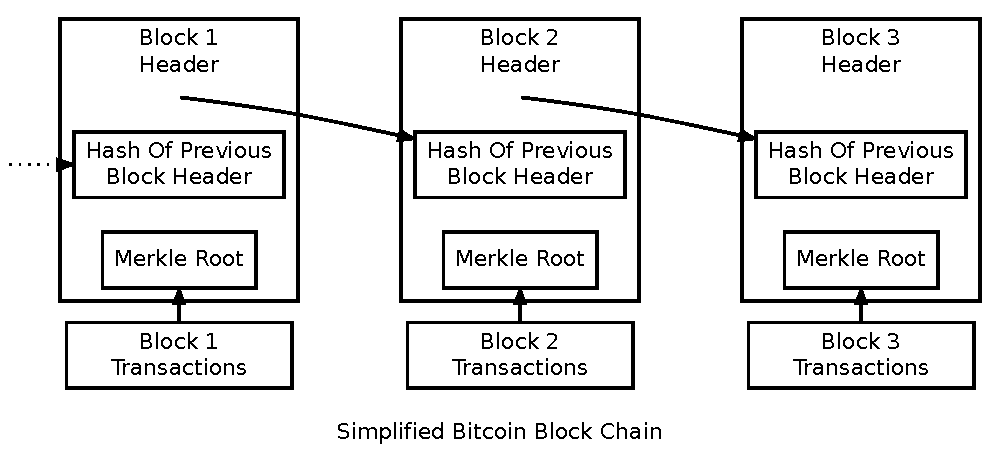
\includegraphics[width=0.9\columnwidth,keepaspectratio]{Images/block-structure.pdf}
  \caption{The block structure~\cite{Nakamoto_bitcoin:a}}
  \label{fig:block-structure}
\end{figure}
\pagebreak

A block header contains mainly the hash of the previous block, a \hyperref[sec:merkle-trees]{Merkle root hash} (see \hyperref[sec:merkle-trees]{section}~\ref{sec:merkle-trees}) to commit to a set of transactions, and a nonce. Blocks are always referenced by the hash of their block header. Once a transaction has been included in a valid block it's called \emph{confirmed}.

\section{\label{sec:blockchain}Blockchain}
Now, the reader can visualize the famous term \emph{blockchain}. The blockchain is a chain of blocks. The blockchain is public and it holds the history of all valid transactions in a cryptocurrency's network. It holds the timeline of a cryptocurrency's life. It is easy to see that, by the definition of the blockchain, there can be no parallel chains. There is not such thing in economics as two valid transaction histories.

It's possible that there are contending chains of blocks. We then say, there is a \emph{fork} on the chain. On \hyperref[fig:blocks]{figure}~\ref{fig:blocks}, the chain has forked on blocks 3 and 6.

We call any valid blocks which are not part of our active chain \emph{orphans}. In our example blocks 4b, 7a and 8a are orphans. As expected, orphans blocks, although typically valid, cannot be part of the transaction history. So, transactions that are included in an orphan block (and have not been included in another block yet) return back in the pool (become \emph{unconfirmed}\footnote{Note: The reader may find this peculiar. However, we observe that as the blockchain grows, older blocks become "safer" (less probability to become orphans). That means that after a transaction becomes confirmed (included in a valid block), one should wait until this valid block is "safe enough".}) and are expected to be included in a block in the future.
\begin{figure}[H]
  \centering
  \includegraphics[width=0.9\columnwidth,keepaspectratio]{Images/blocks.png}
  \caption{A blockchain (the orange blocks are orphans)~\cite{mastering}}
  \label{fig:blocks}
\end{figure}

\section{Proof of Work (PoW)} \label{sec:proofofwork}
The key to making Bitcoin decentralized is a technique called Proof of Work (PoW). Proof of Work was first invented in 1992 by Dwork et al.~\cite{dwork} as a measure of limiting email spam and denial of service attacks and later explored by Back~\cite{hashcash} as Hashcash.

We'll examine a simplified model of Hashcash in order to explore the idea. Suppose we want to send an email to someone. In order to prove we've done work, we include a header (like \code{X-Hashcash}), which includes the receiver's email address, and a nonce\footnote{Hashcash headers actually contain 7 different fields which have been omitted here for simplicity. The simplified version explained here is not making the same security guarantees as Hashcash.}. The nonce is picked so that the hash of the header $H(email || nonce)$ has its 20 most significant bits be all 0. The only feasible way to find this is by brute-forcing the nonce. Once the sender has found the nonce, it's included in the header and sent.

The receiver can then very easily check whether the header hashes to a valid value. If that's so, the email it contains belongs to the receiver and the header is not being reused. After this confirmation, the email can be considered not spam.

To reiterate, the idea is having a series of data to commit to and a hole for the nonce, which is brute-forced to satisfy a necessary predicate on the hash, specifically that its $n$ most significant bits are all zeroes. This is exactly how Bitcoin implements Proof of Work. Instead of the hole being on an email header the hole is on the block header. For a block to be valid, its header has to satisfy a predicate like the above.

Bitcoin introduces a couple of differences. $n$ varies according to the block generation rate. Specifically, to translate the previous predicate to Bitcoin terminology, the hash of each block header has to satisfy
\begin{equation} \label{eq:PoW}
  H({\sf blockHeader}) \le T
\end{equation}
where $T$ is called the \emph{target}. As the target goes up, the probability of being below it goes up and generating a valid block is easier. Conversely, if the target goes down it's harder to generate a valid block. To express this, in Bitcoin, $\frac{1}{T}$ is called the \emph{difficulty}.

To account for the block generation rate, which Bitcoin tries to keep to 1 block per 10 minutes, every 2016 blocks the target (and subsequently the difficulty) is adjusted accordingly. The target is calculated inside the Bitcoin software and is only a function of the blocks previously seen (frequently called their \emph{view}). So, as long as the Bitcoin nodes agree on the view, they'll agree on the target and all will consider the same set of incoming blocks as valid.

\section{Simplified Payment Verification (SPV)}
The size of the blockchain has reached 197GB by the beggining of January 2019, which makes it a very time consuming or even infeasible process to synchronise a full node. Fortunately, a solution was proposed in the original white paper ~\cite{Nakamoto_bitcoin:a}, which allows the creation of so-called \emph{lite nodes}.

Lite nodes only know the headers of the entire blockchain, which are constant-size for each block (80 bytes). At the time of writing of this thesis, the size of all block headers was $\sim$45MB. The lite node then asks the network for transactions concerning it (e.g. transactions concerning a specific public key). Full nodes of the network find such transactions and return them to the requester. For each transaction, the block header of the block it is included in, is returned along with a \hyperref[sec:merkle-trees]{Merkle tree} (see \hyperref[sec:merkle-trees]{section}~\ref{sec:merkle-trees}) proof of inclusion which the lite node can then verify.

This protocol is reliable, as long as an adversary does not control the network of a lite node.

%%%%%%%%%%%%%%%%%%%%%%%%%%%%%%%%%%%%%%%%%%%%%%%%%%%%%%%%%%%%%%%%%%%%%%%%%%%%%%%%
%%%%%%%%%%%%%%%%%%%%%%%%%%%%%%%%%%%%%%%%%%%%%%%%%%%%%%%%%%%%%%%%%%%%%%%%%%%%%%%%
%%%%%%%%%%%%%%%%%%%%%%%%%%%%%%%%%%%%%%%%%%%%%%%%%%%%%%%%%%%%%%%%%%%%%%%%%%%%%%%%
